\documentclass[a4paper]{article}
\usepackage[12pt]{extsizes}
\linespread{1.3}
\usepackage[warn]{mathtext}
\usepackage[utf8]{inputenc}
\usepackage[T2A]{fontenc}
\usepackage[english,russian]{babel}
\usepackage{booktabs}
\usepackage{multicol}
\usepackage{fancyhdr}
\usepackage{graphicx}
\usepackage{microtype}
\usepackage{wrapfig}
\usepackage{amsmath}
\usepackage{floatflt}
\usepackage{geometry} 
\usepackage{float}
\usepackage{amssymb}
\usepackage{caption}
\usepackage{epsfig}
\usepackage{newunicodechar}
\usepackage{color}

\geometry{verbose,a4paper,tmargin=2cm,bmargin=2cm,lmargin=3cm,rmargin=1.5cm}


\begin{document}

\graphicspath{ {pictures/} }

\tableofcontents
\newpage

\section{Введение}

Радиоастрономия является основным движителем развития сверхчувствительных смесителей для гетеродинных приемников электромагнитного излучения 
миллиметровых и суб-миллиметровых длин волн. Смесители на основе туннельного перехода сверхпроводник – изолятор – сверхпроводник (СИС) \cite{Tucker} 
имеют рекордные шумовые характеристики в этом диапазоне, близкие к квантовому пределу. Среди наземных приемников наибольшее распространение получили 
смесители с разделением боковых полос, которые имеют в составе два одиночных СИС-смесителя \cite{Belitsky} \cite{Chenu}. 
\par

Для эффективной работы 
приемника, а именно для достижения предельной чувствительности и для высокого качества разделения боковых полос, принципиально важно иметь СИС-смесители 
с низким уровнем отражения. Низкий уровень отражений нужен как по входу смесителя, т.е. на частоте принимаемого сигнала, на высокой частоте (ВЧ) 
\cite{Hesper} \cite{Khudchenko}, так и по выходу, т.е. на промежуточной частоте (ПЧ, IF). В тракте ПЧ такая необходимость обусловлена возникновением 
стоячих волн между самим СИС-смесителем и криогенным малошумящим усилителем, так как последний имеет достаточно высокий уровень отражения до $\sim -6$ дБ.
\par

Данная работа посвящена определению уровня отражений от 
СИС-смесителя в рабочем режиме с целью минимизации этого уровня в будущем. Для решения поставленной задачи проведен теоретический расчет уровня 
отражения от СИС-смесителя по выходному тракту ПЧ, а также собрана экспериментальная схема, и проведено непосредственное измерение отраженного сигнала.
\par 

Полученные результаты могут быть применимы для лучшей характеризации СИС-смесителей и оптимизации их работы.


\newpage
\section{Литобзор}

На данный момент достаточно много научных статей, посвященных изучению криогенных приемников на основе туннельного перехода СИС и их различных характеристик.
Однако, на настощий момент нет опубликованных материалов и результатов экспериментов с прямым измерением уровня отражения по промежуточной частоте от СИС-смесителя.
\par

В работе Serres et al. \cite{Serres}, посвященной определению выходного импеданса СИС-смесителя по промежуточной частоте, приведено сравнение теоретических 
рассчетов и экспериментальных результатов. Цель данной статьи достаточно близка к нашей, по скольку определение импеданса необходимо для получения уровня отражения.
Предложена модифицировання однопортовая экспериментальная схема с использованием циркулятора.
Особенностью калибровки является то, что сам СИС-сместель используется как калибратор, двигаясь по его вольт-амперной характеристике (ВАХ) можно получить три калибрововчных стандарта (SOL).
Причем, такая калибровка позволяет учесть собственную емкость и индуктивность перехода.
Численный рассчет импеданса смесителя опирается на теорию Tucker et al. \cite{Tucker}.
\par 

\subsection{Теоретическое описание}

Величина отражений от СИС-смесителя по тракту ПЧ, характеризуемая параметром $S11_{IF}$  \cite{Kooi}, может быть определена, если известен выходной импеданс ПЧ СИС-смесителя $Z_{IF}$  и импеданс подводящей линии тракта ПЧ $Z_L$
\begin{equation}
    S11_{IF} = \frac{Z_{IF} - Z_L}{Z_{IF} + Z_L}
    \label{s11}
\end{equation}
Для расчета  мы используем 3х частотное приближение к теории квантового смешения Tucker \cite{Tucker}. Рассмотрены сигналы на частотах 
$f_m = m \cdot f_{LO} + f_0$, 
где $m = 0, \pm 1$; $f_{\pm}$  - верхняя и нижняя полосы; $f_{LO}$ - частота опорного генератора; $f_0$ - промежуточная частота. Полагаем, что более высокие гармоники шунтируются емкостью СИС-смесителя, составляющей в нашем случае порядка 100 фФ.
Принимая во внимание взаимодействие портов смесителя, компоненты напряжений и токов слабых сигналов линейно связаны матрицей проводимости $i_m = \sum_{m'} Y_{mm'}' \upsilon_{m'} $ :
\begin{equation}
    Y_{mm'}' (V_{gap}, R_N, f_{LO}, \alpha, V_0) = 
    \begin{bmatrix}
        Y_{11} + Y_{S} & Y_{10} & Y_{1-1}  \\
        Y_{01} & Y_{00} + Y_L & Y_{0-1}   \\
        Y_{-11} & Y_{-10} & Y_{-1-1}+Y_I  \\
    \end{bmatrix}
    \label{Y_mm}
\end{equation}
где $V_{gap}$ - напряжение смещения туннельного скачка тока, $R_N$ - нормальное дифференциальное сопротивление ВАХ, $\alpha = e V_{LO} / h f_{LO}$ - безразмерный параметр накачки, 
пропорциональный напряжению опорного генератора $V_{LO}$ , $V_0$ - напряжение смещения СИС-смесителя.
\par

У каждого порта есть своя канальная проводимость: $Y_1 = Y_S$ - нагрузка порта с принимаемым сигналом, $Y_0 = Y_L$ - нагрузка порта ПЧ, $Y_{-1}=Y_I$ - нагрузка порта нижней полосы.
\begin{figure}[H]
    \begin{center}
        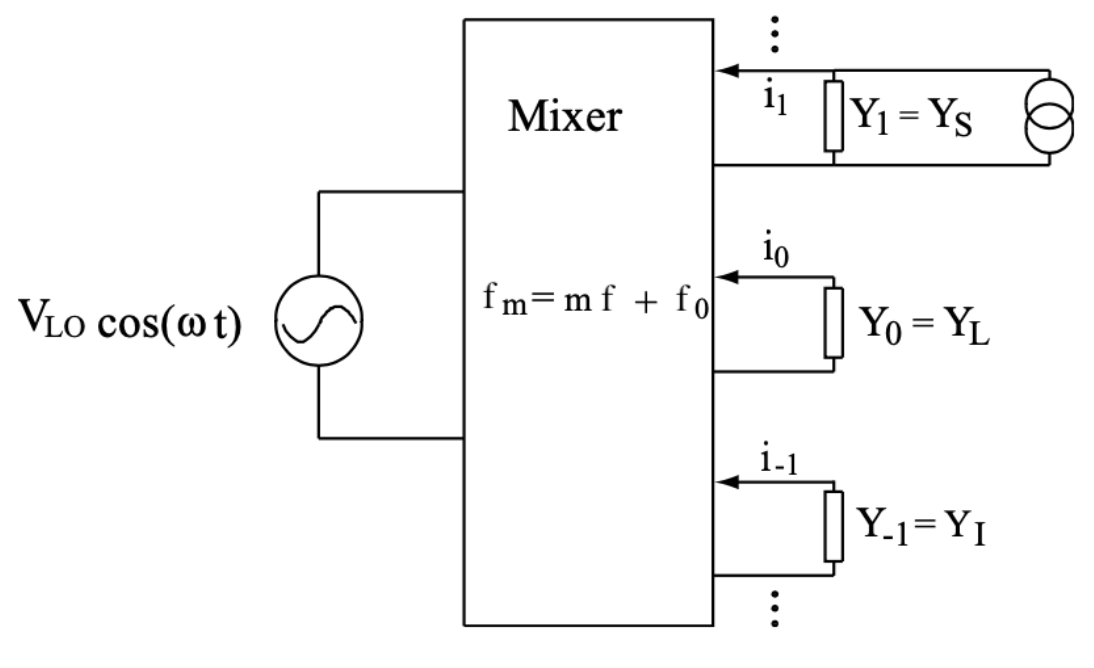
\includegraphics[scale=0.5]{mixer_scheme.png}
        \caption{Эквивалентная схема гетеродинного смесителя, с приложенным сигналом опорного генератора частоты , принимаемым сигналом частоты  и сигналом ПЧ}
        \label{mixer_scheme}
    \end{center}
\end{figure}

Для  идеального двухполосного  смесителя  импедансы верхней и нижней полос равны $Y_1 = Y_{-1}$. В нашем случае $Y_{\pm 1}$ - результат преобразования проводимости  опорного генератора несколькими микрополосковыми линиями.
\par 

Воспользовавшись результатом \cite{Tucker}, получим $Y_{mm'} = G_{mm'} + i B_{mm'}$ , где

\begin{equation}
    \begin{split}
    G_{mm\prime} = \frac{e}{2 \hbar \omega_{m\prime}} 
    \cdot \sum_{n,n\prime=-\infty}^{\infty} J_n(\alpha) J_{n\prime}(\alpha) \delta_{m-m\prime, n\prime-n} \\
    \left\{ \left[ I_{dc}(V_0+n\prime \hbar \omega /e + \hbar \omega_{m\prime}/e) - 
    I_{dc}(V_0 + n\prime \hbar \omega/e) \right] + \right. \\
    \left. \left[ I_{dc}(V_0 + n\hbar \omega/e) - 
    I_{dc}(V_0 + n \hbar \omega/e - \hbar \omega_{m\prime}/e) \right]  \right\}
    \end{split}
\end{equation}

\begin{equation}
    \begin{split}
        B_{mm\prime} = \frac{e}{2 \hbar \omega_{m\prime}} \cdot 
        \sum_{n,n\prime=-\infty}^{\infty} J_n(\alpha) J_{n\prime}(\alpha) \delta_{m-m\prime, n\prime-n} \\
        \left\{ \left[ I_{kk}(V_0+n\prime \hbar \omega /e + \hbar \omega_{m\prime}/e) - 
        I_{kk}(V_0 + n\prime \hbar \omega/e) \right] - \right. \\
        \left. \left[ I_{kk}(V_0 + n\hbar \omega/e) - 
        I_{kk}(V_0 + n \hbar \omega/e - \hbar \omega_{m\prime}/e) \right]  \right\}
    \end{split}
\end{equation}

Где $I_{dc}(V_0)$ - зависимость туннельного тока СИС-смесителя от его напряжения; $I_{kk}(V_0)$ - зависимость соотношения Крамерса-Кронига тока $I_{dc}$ от напряжения СИС-смесителя; 
$J_n(\alpha)$ - функция Бесселя порядка  от параметра накачки $\alpha$ .
Тогда, в нашем случае импеданс по ПЧ:
\begin{equation}
    Z_{IF} = \left \| Y_{mm'} + Y_{m} \delta_{mm'} \right \|^{-1}_{00} 
\end{equation}

На рис.\ref{pic-IV} продемонстрирована измеренная ВАХ СИС-перехода, которая является зависимостью $I_{dc}(V_0)$ и определяет $I_{kk}$. 
Автономная кривая показана зеленой линией, при этом, оранжевой кривой показана ВАХ для случая, когда приложен внешний сигнал генератора частотой 600 ГГц. 

\begin{figure}[H]
    \begin{center}
        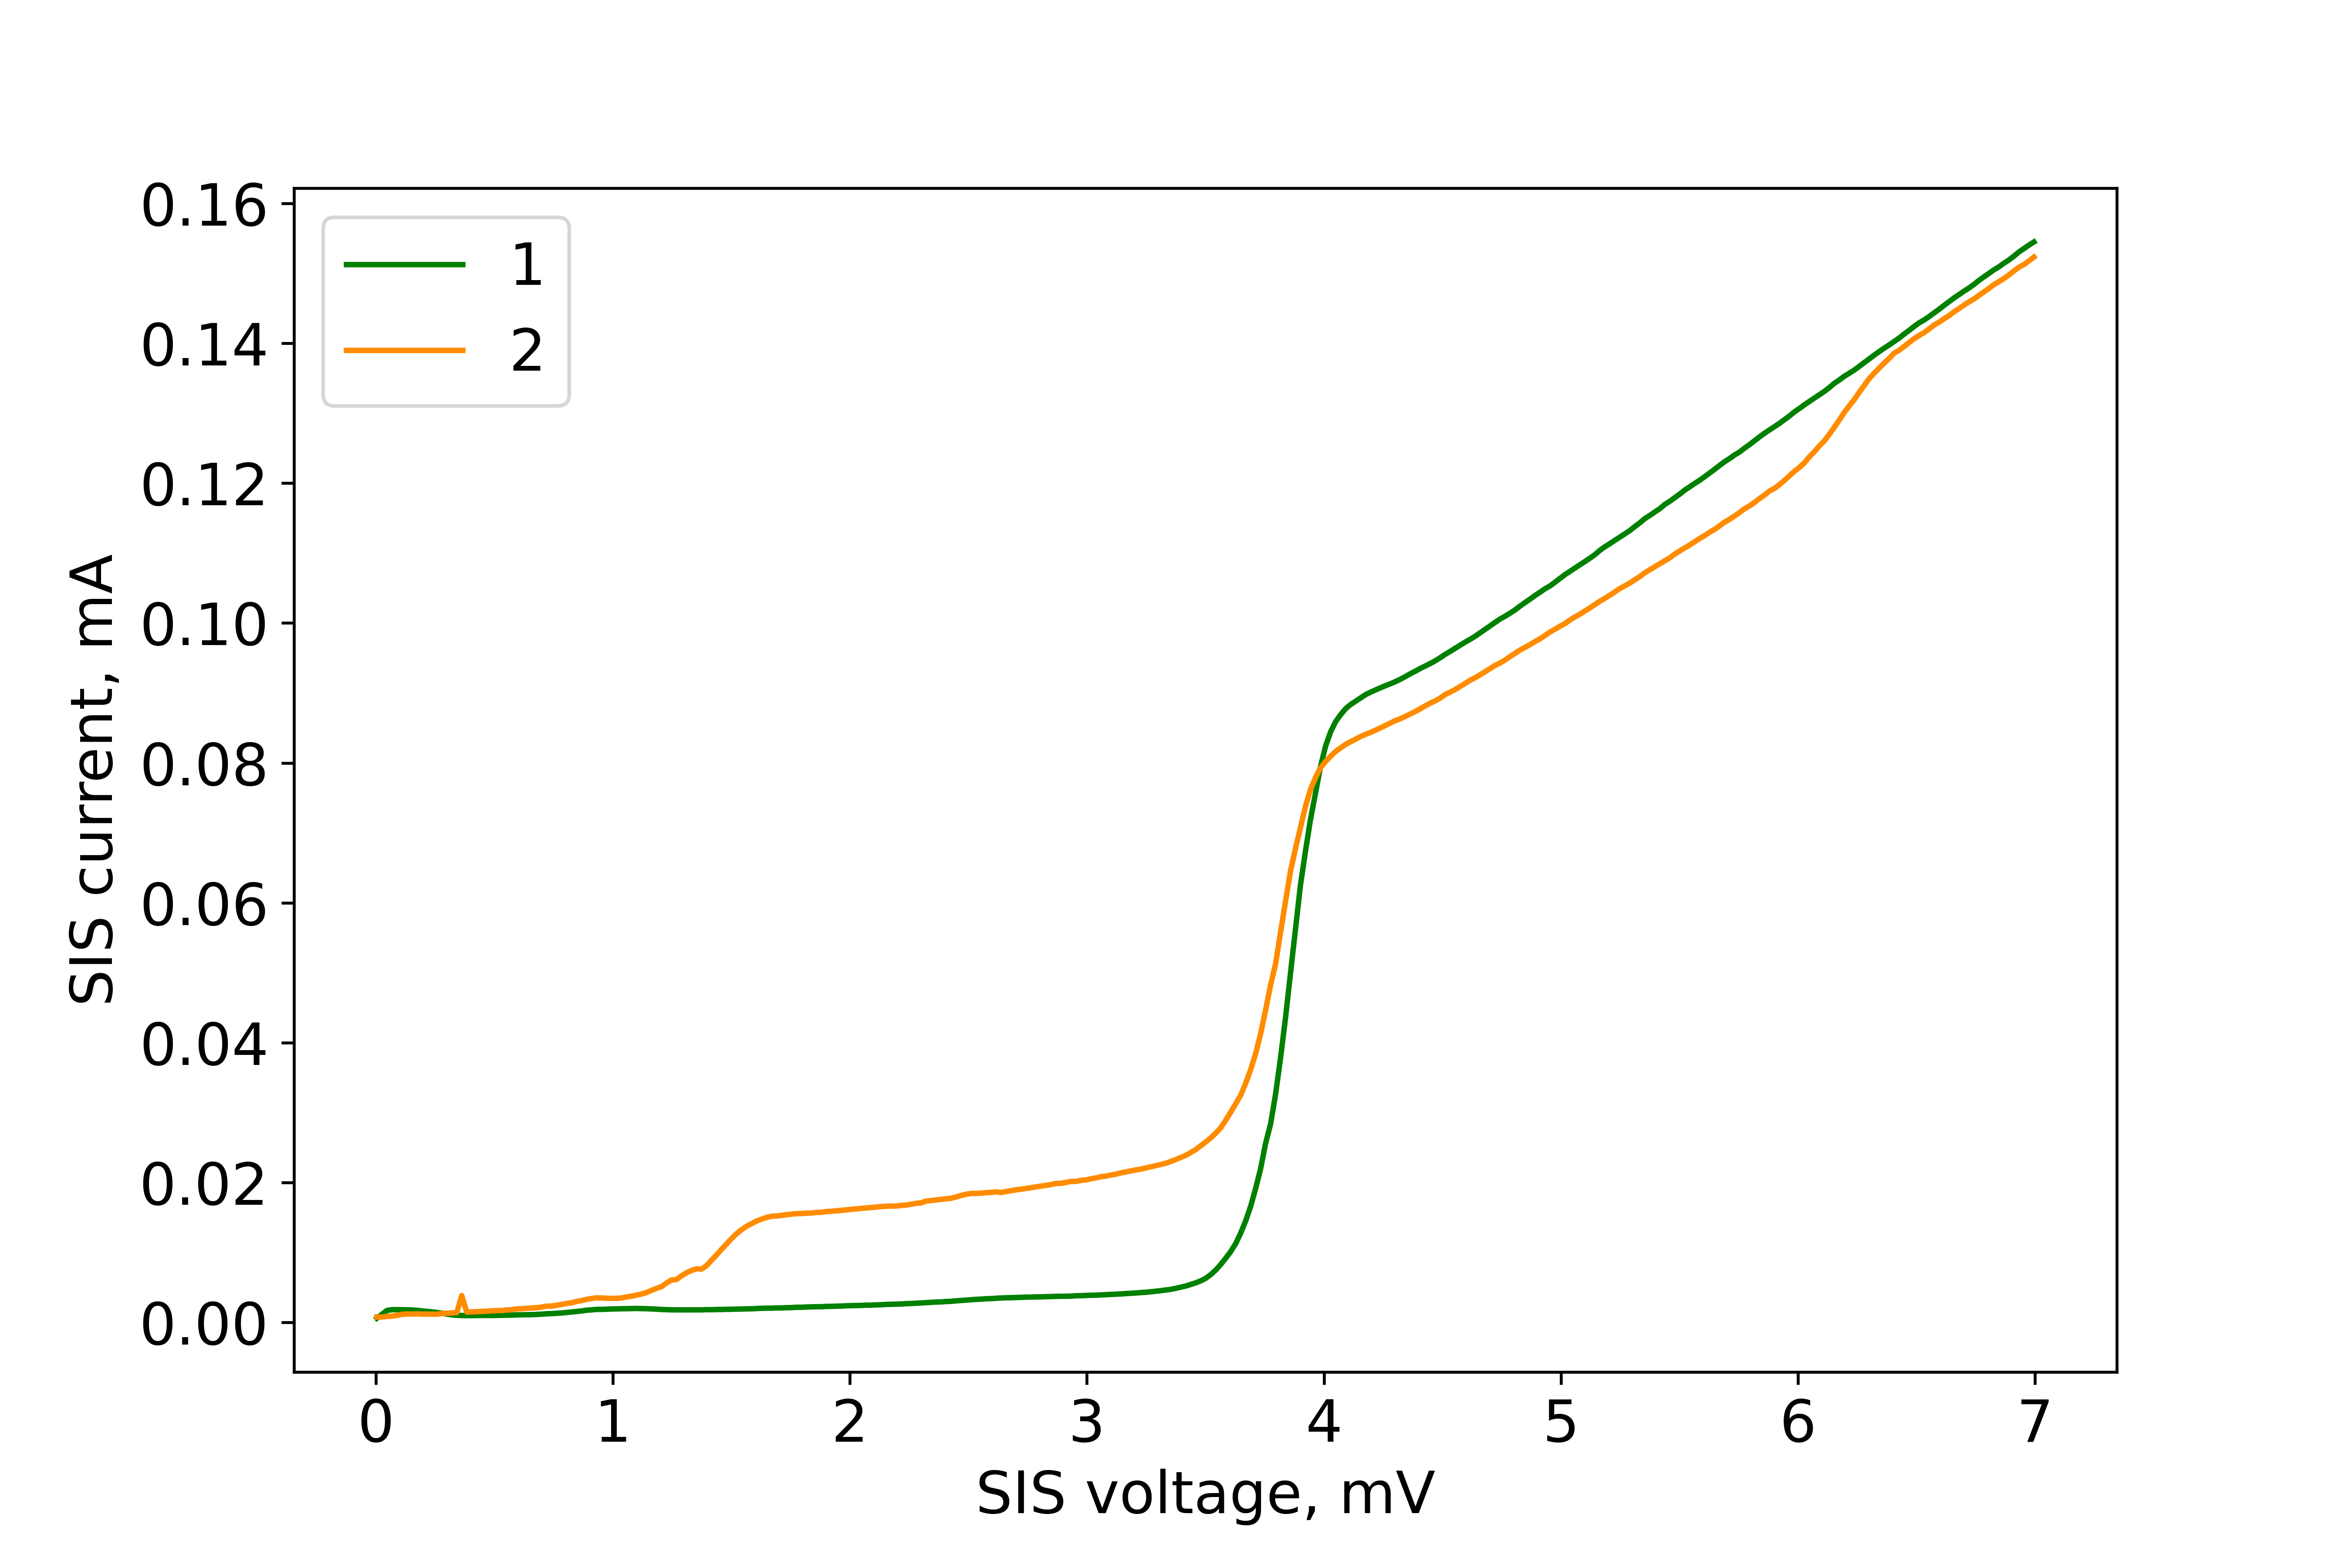
\includegraphics[scale=0.5]{IV.png}
        \caption{ВАХ автономная (№1 зеленая кривая) и с приложенным сигналом опорного генератора (№2 оранжевая кривая).}
        \label{pic-IV}
    \end{center}
\end{figure}

На рис.3 приведен результат теоретического расчета импеданса с использованием ВАХ (рис.\ref{pic-IV}) в диапазоне ПЧ 0.1-12 ГГц при различных напряжениях на СИС-переходе: 2.8, 3, 3.2 мВ, 
причем импеданс подводящей линии полагается $\sim 50$ Ом. Можно заключить, что действительная часть изменяется незначительно с промежуточной частотой, в отличие от мнимой части. 
Также видно, что импеданс сильно зависит от напряжения на СИС-переходе.

\begin{figure}[H]
    \begin{center}
        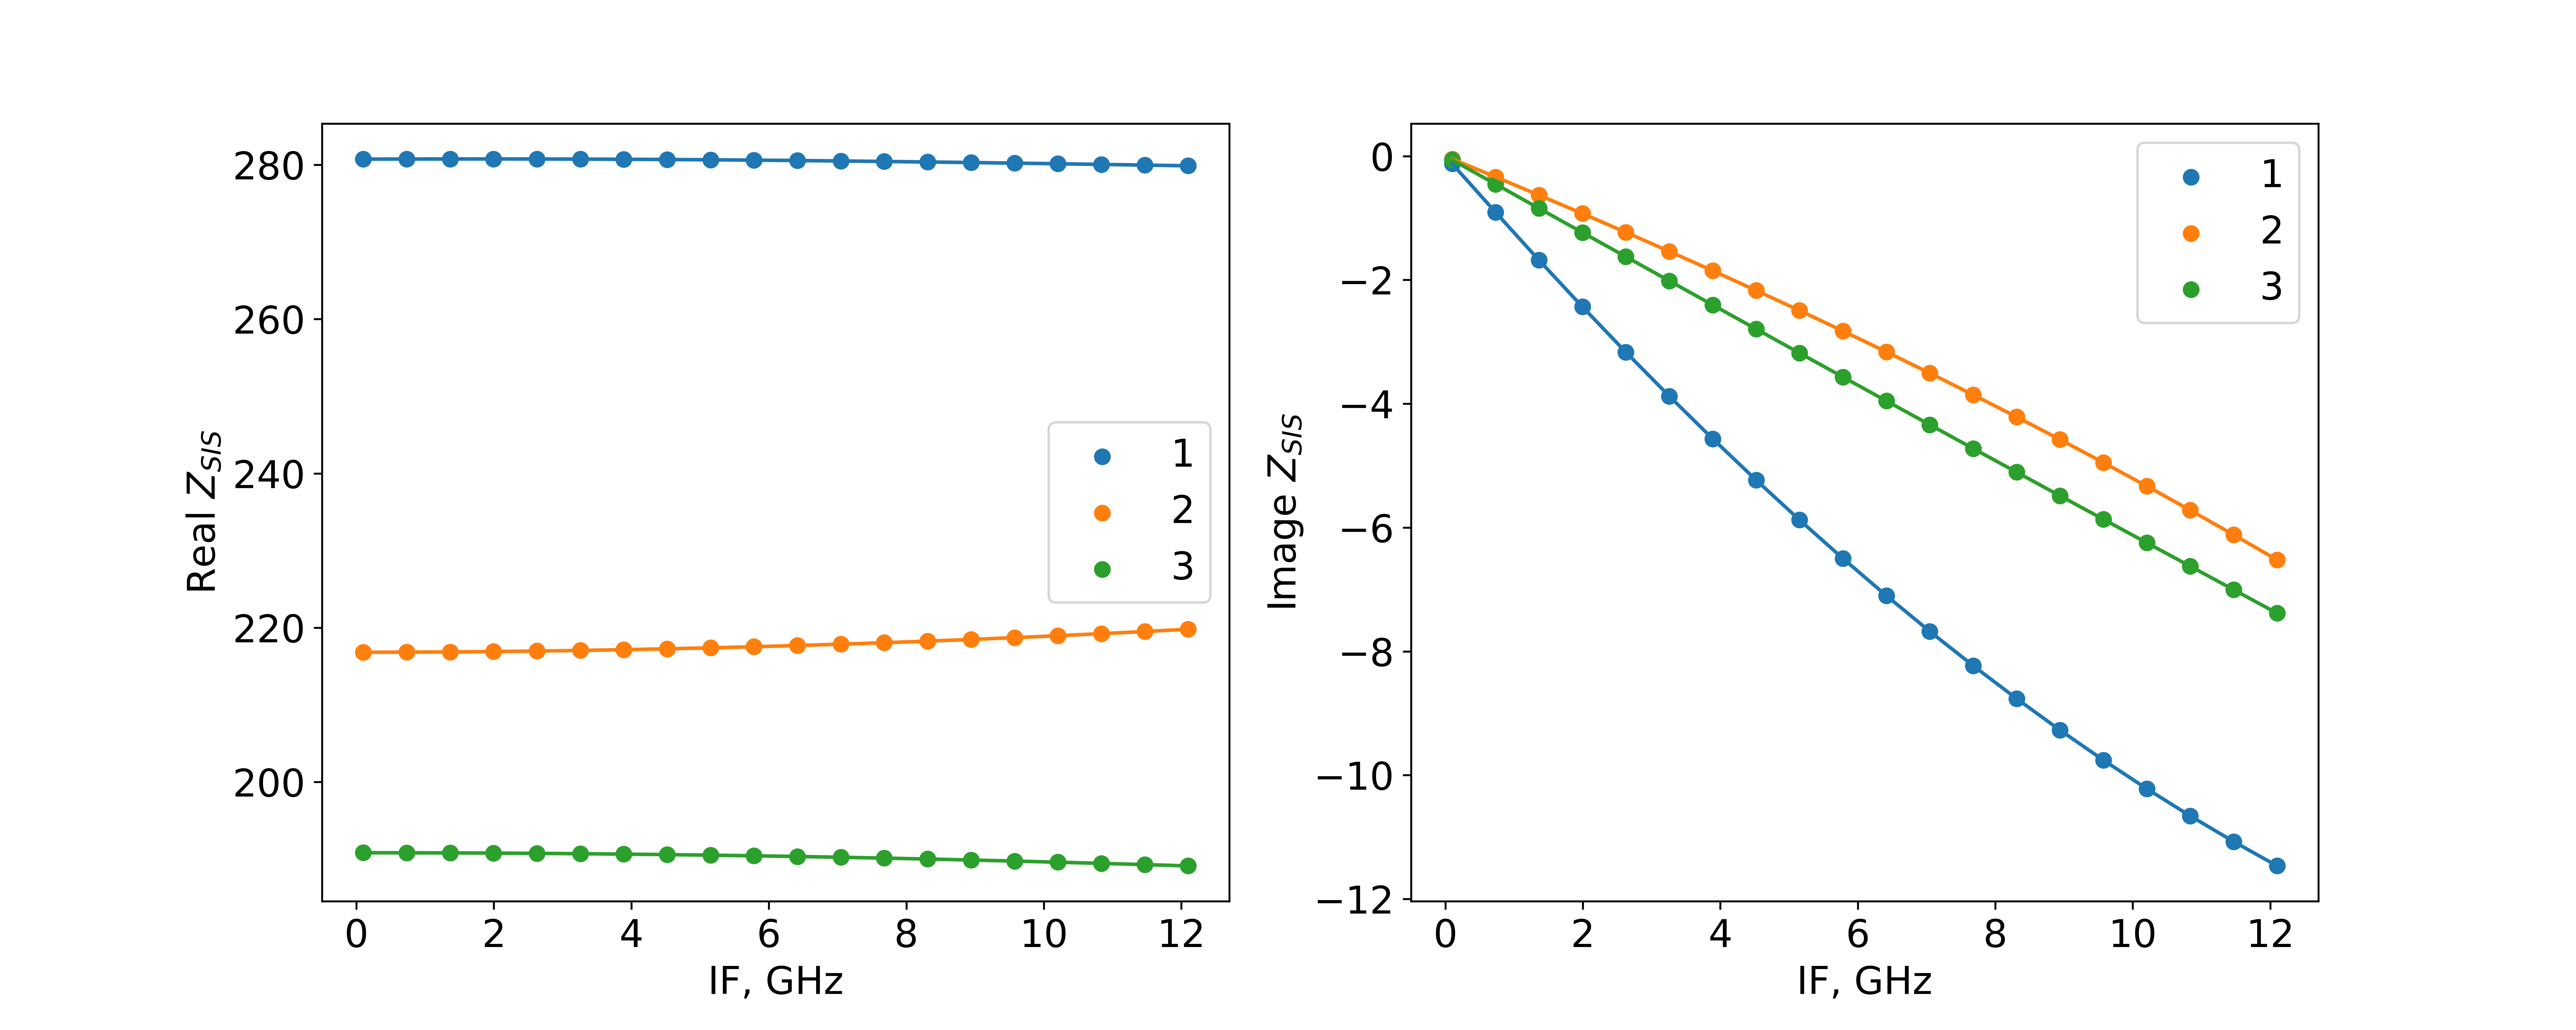
\includegraphics[scale=0.5]{reim.png}
        \caption{Действительная (слева) и мнимая (справа) части расчетного импеданса СИС-смесителя от ПЧ при разных напряжениях на СИС-смесителе; №1 – 2.8 мВ, №2 – 3 мВ, №3 – 3.2 мВ.}
        \label{pic-reim}
    \end{center}
\end{figure}


\subsection{Постановка эксперимента}
Задача эксперимента - измерение уровня отражения от СИС-смесителя по выходному каналу ПЧ, когда на смеситель подается напряжение смещения и приложен сигнал высокочастотного опорного генератора. 
Измерения проведены в диапазоне 4–8 ГГц; этот диапазон определен полосой используемого криогенного ПЧ усилителя. Схема эксперимента представлена на Рис.\ref{pic-setup}; 
СИС-смеситель помещен в криостат замкнутого цикла при температуре около 4 K. Высокочастотный опорный генератор (LO) интегрирован с СИС-смесителем на одном 
чипе и представляет собой распределенный джозефсоновский переход c вязким течением магнитных вихрей (РДП, FFO).  Векторный анализатор цепей (ВАЦ, VNA), 
размещенный вне криостата, генерирует тестовый сигнал диапазона 4–8 ГГц на порте (П1, P1), который, проходя через аттенюатор -10 дБ, поступает в направленный 
ответвитель (Directional coupler), который направляет его на СИС-смеситель с коэффициентом связи около -10 дБ. Далее сигнал проходит специальный инжектор (Bias Tee), 
позволяющий беспрепятственно проходить ПЧ сигналу, задавая при этом напряжение на СИС-смесителе по постоянному току через большую индуктивность. 
Отразившись от СИС-смесителя, основная часть сигнала проходит напрямую через направленный ответвитель и поступает на вход криогенного малошумящего усилителя (LNA), 
который усиливает этот сигнал и направляет его на приемный порт (П2, P2) ВАЦ. Фактически, измеряемым параметром является отношение сигналов ВАЦ на портах П1 и П2, а точнее его спектр.

\begin{figure}[H]
    \begin{center}
        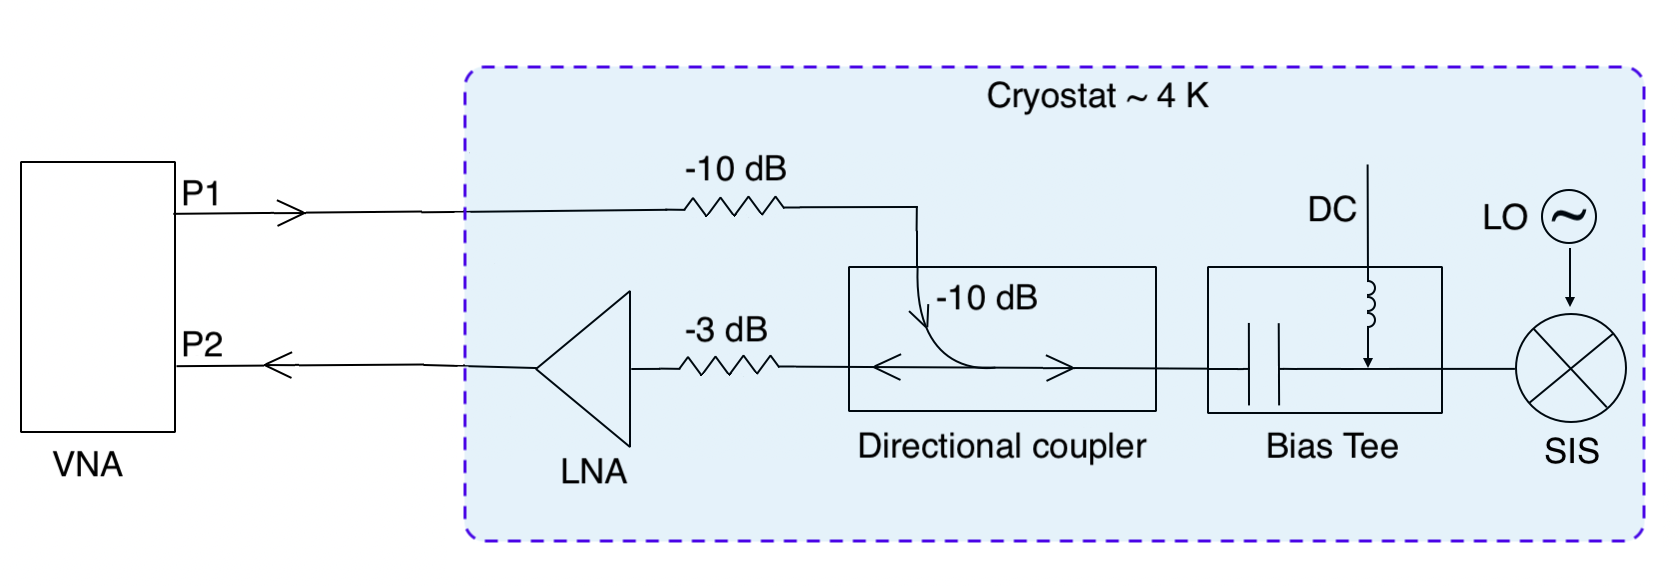
\includegraphics[scale=0.5]{setup.png}
        \caption{Схема эксперимента по измерению отражения от СИС-смесителя по выходу ПЧ}
        \label{pic-setup}
    \end{center}
\end{figure}


\subsection{Калибровка}
Важным этапом в эксперименте является калибровка ВАЦ, чтобы повысить точность измерений. Мы используем стандартную однопортовую калибровку (Рис. \ref{pic-error}), 
в основе которой лежит определение 3х параметров цепи: D - прямые утечки в цепи, R - внутренние отражения, M - рассогласование. Путем несложных преобразований, 
можно явно выразить фактический коэффициент отражения $\Gamma$  через измеряемую величину $\Gamma_m$ и 3 калибровочных параметра D, R, M:

\begin{equation}
    \Gamma = \frac{\Gamma_m - D}{R + M(\Gamma_m - D)}
    \label{gamma}
\end{equation}

Коэффициенты D, R, M могут быть определены по трем калибровочным измерениям, путем составления и решения системы из трех уравнений (\ref{gamma}), где коэффициент отражения  вычисляется теоретически по формуле (1), а величина  непосредственно измеряется векторным анализатором цепей.

\begin{figure}[H]
    \begin{center}
        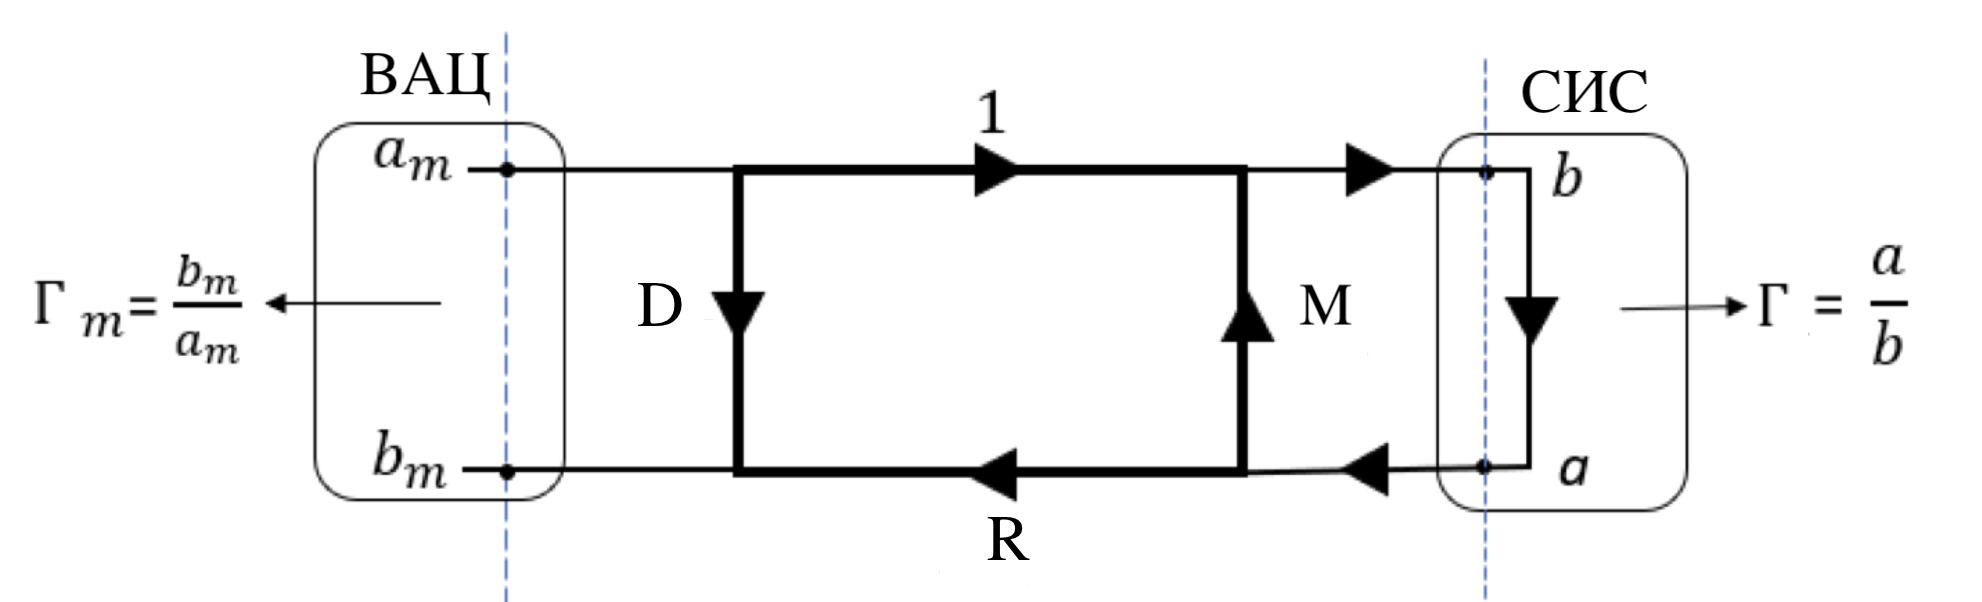
\includegraphics[scale=0.5]{Error.png}
        \caption{Схема однопортовой калибровки.}
        \label{pic-error}
    \end{center}
\end{figure}

В калибровочных измерениях при 4 К сам СИС-переход используется как калибратор \cite{Serres}. Это позволяет избежать погрешностей, возникающих при калибровке при 
комнатной температуре и связанных с изменениями электрической длины и импеданса элементов цепи при охлаждении. СИС-смеситель находится в автономном 
состоянии, т.е. без приложения внешнего сигнала. 


На Рис. \ref{pic-cal} проиллюстрировано, какие напряжения смещения используются для калибровки:  1) при напряжении смещения в 2 мВ  дифференциальное сопротивление 
становится порядка 1000 Ом, что близко к ситуации «открытой цепи», т.к. импеданс подводящей линии близок к величине  Ом; 2) при напряжении смещения 3.8 мВ, 
т.е. посередине туннельного скачка тока, его дифференциальное сопротивление составляет около 3 Ом, что приближенно соответствует калибровке «короткое замыкание»; 
3) при напряжении смещения 5–7 мВ дифференциальное сопротивление становится  Ом, что близко к ситуации «нагруженной линии». 

\begin{figure}[H]
    \begin{center}
        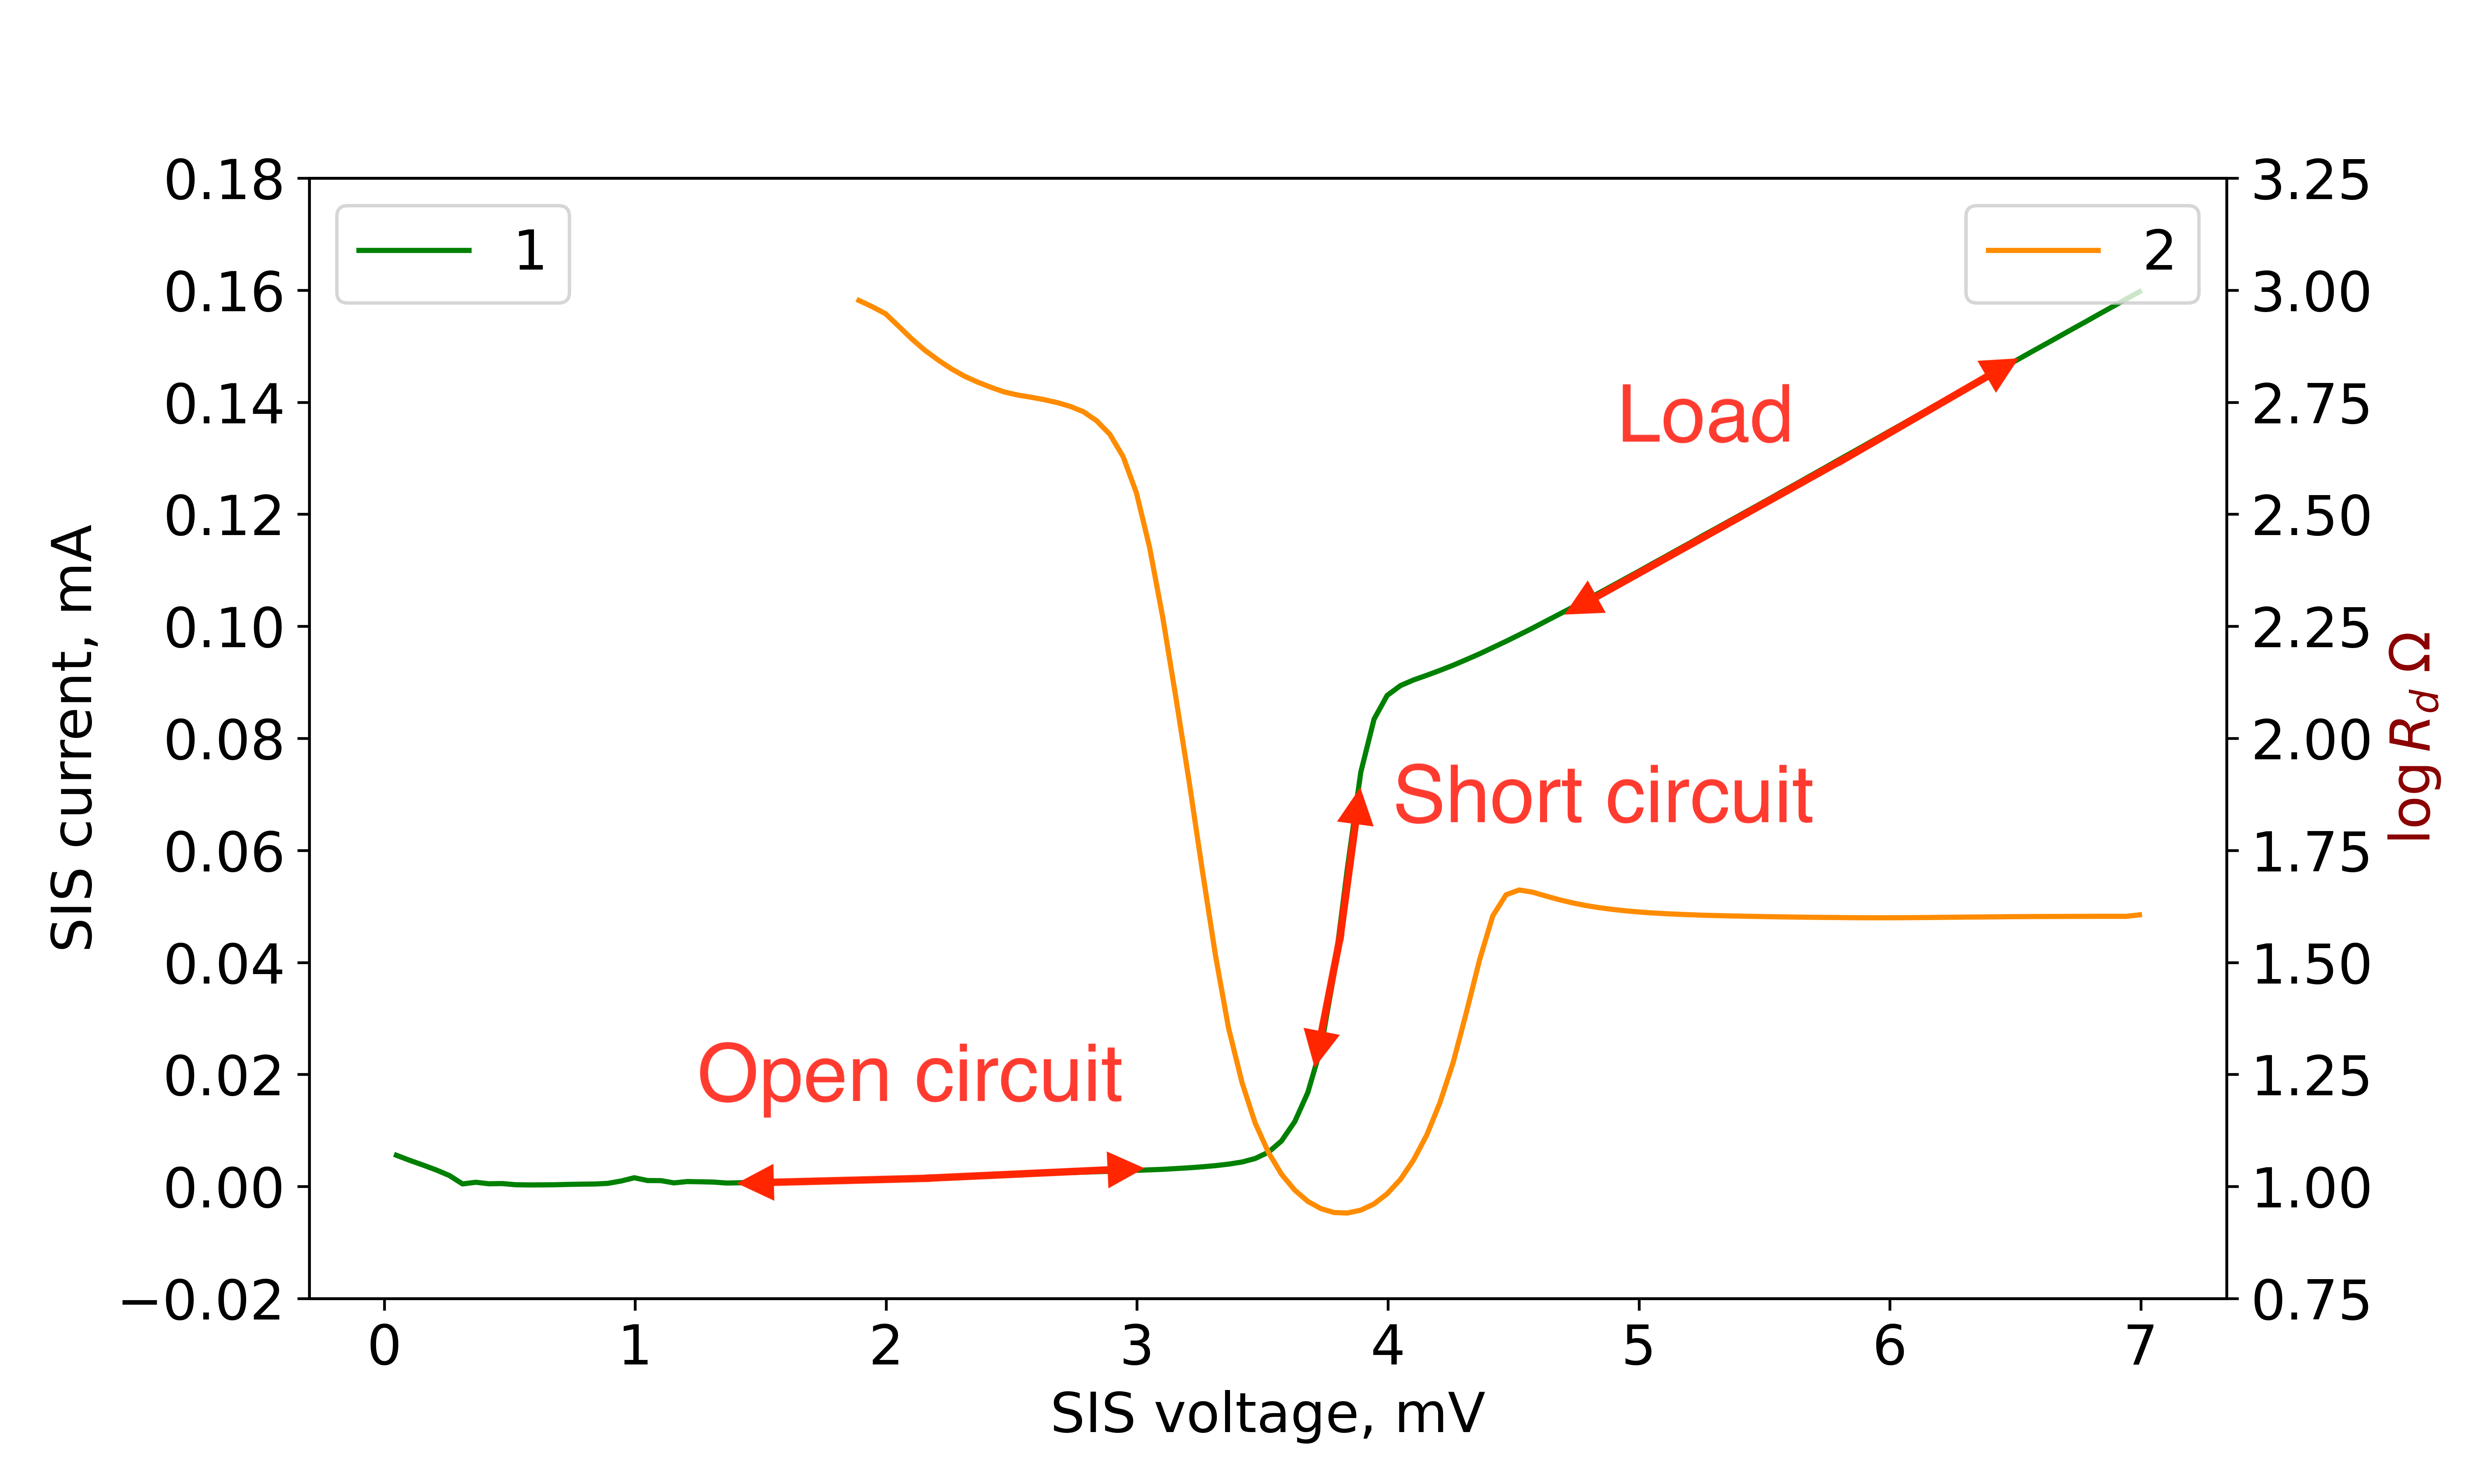
\includegraphics[scale=0.5]{cal.png}
        \caption{Автономная Вольт-амперная характеристика СИС-смесителя №1 зеленая линия; соответствующее дифференциальное сопротивление показано оранжевой линией №2.}
        \label{pic-cal}
    \end{center}
\end{figure}


Этих трех калибровок достаточно, чтобы составить 3 уравнения используя (\ref{gamma}) и тем самым определить коэффициенты D, R и M. Это позволяет учесть все отражения и 
утечки в цепи и корректно измерить отражение от СИС-смесителя в рабочем режиме. Стоит отметить, что в приведенной калибровке внутренняя емкость СИС-смесителя выступает 
как часть внешней цепи и ее влияние также нивелируется калибровкой.

% \newpage
% \section{Результаты}
%  ВАХ СИС-смесителя, при приложении сигнала опорного генератора частотой  ГГц в «рабочем» режиме, показана на рис.1  оранжевой кривой. Диапазон «рабочего» напряжения смещения лежит приблизительно в интервале 1.6–3.4 мВ. Эта область напряжений соответствует так называемой квазичастичной ступени, вызванной приложением к СИС-переходу сигнала гетеродина. На рис.7 приведены экспериментальные (непрерывные кривые) и теоретические (пунктирные кривые) частотные зависимости уровня отражения при различных напряжениях на СИС-смесителе. Из приведенных результатов видно, что в диапазоне 4–8 ГГц уровень отражения почти не меняется с частотой, что хорошо согласуется и с теоретическими предсказаниями. 

% Рис. 7. Рассчитанный теоретически (№ 1,2 пунктирные линии) и определенный экспериментально (№ 3,4 сплошные кривые) уровень отражения от СИС-перехода в «рабочем режиме»; Напряжения СИС-смесителя № 1,3 –  2 мВ, № 2,4 – 2.6 мВ
% Изменение уровня отражений при варьировании напряжения смещения СИС-смесителя продемонстрировано на Рис.8. Здесь приведены результаты измерений и расчета отражения для середины диапазона ПЧ, а именно при частоте 6 ГГц. Синие точки - экспериментальные данные, красная сплошная кривая – теоретический расчет. Уровень отражения в среднем составляет около 4 дБ. При напряжении около 2 мВ имеет место искажение ВАХ вызванное краем джозефсоновской ступени, которая проявляется ввиду наличия неподавленного критического тока перехода. Это искажение вызывает аномалию в уровне отражения.  Можно заметить, что при напряжении 3.5 мВ уровень отражения значительно снижается (детально на Рис.9). Этот пик поглощения можно объяснить тем, что импеданс СИС-смесителя становится почти равным  импедансу подводящей линии ПЧ, формула (1). Точнее, в этой точке дифференциальное сопротивление СИС-смесителя становится равным действительной компоненте импеданса подводящей линии .  Вычислив импеданс СИС-смесителя по формуле (3) мы сможем экспериментально определить импеданс подводящей линии . В данном случае, мы наблюдаем, что  с высокой степенью точности составляет  Ом. На Рис.9 приведено сравнение экспериментального уровня отражения и теоретического. Важно отметить, что уровень отражения в минимуме определяется модулем разности мнимых компонент импедансов СИС-смесителя и подводящей линии. Отличие глубины пика поглощения в измерении и в расчете позволяет проверить достоверность расчета, а также оценить величину комплексной части импеданса подводящей линии и за счет проведения измерений при различных частотах ПЧ. В нашем случае можно заключить, что мнимая часть импеданса подводящей линии не превышает 2 Ом. Таким образом, предложен и апробирован способ нахождения импеданса подводящей линии, используя особенности ВАХ СИС-смесителя.
% В целом, можно заключить, что уровень отражения достаточно высокий и составляет в среднем около -4.5дБ в «рабочем» диапазоне, что вынуждает нас использовать специальные вентили в канале ПЧ в СИС приемниках для минимизации стоячих волн в тракте ПЧ.

 
% Рис. 8. ВАХ СИС-смесителя: автономная (№ 1 зеленая кривая), нагруженная сигналом опорного генератора (№ 2 оранжевая кривая). Теоретический расчет отражения (№ 3 красная кривая). Результаты измерений отражения (№ 4 синие точки). ПЧ равна 6 ГГц.

% Рис. 9. Уровень отражения в «яме». Точки (№ 1,2,3) - экспериментальный уровень отражения для ПЧ 4,6,8 ГГц соответсвенно; Сплошные кривые (№ 4,5,6) - теоретический расчет уровня отражения для ПЧ 4,6,8 ГГц соответсвенно.

% \newpage
% \section{Заключение}
% Представлен метод экспериментального и теоретического определения ПЧ параметров СИС-перехода. Это позволяет исследовать зависимость уровня отражений от СИС-смесителя по ПЧ выходу от напряжения смещения и от мощности опорного сигнала. Определение параметров самого СИС-перехода совмещенное с моделированием элементов ПЧ канала позволит в будущем рассчитать с высокой точностью ПЧ характеристики самого смесителя, а также всего приёмника сконструированного на его основе. Дополнительная калибровка по пику поглощения при варьировании напряжения смещения позволяет повысить точность измерений, которые хорошо совпадают с теоретическим расчетом.
% В дальнейшем планируется исследование ПЧ параметров на частотах 4-12 ГГц и выше, а также при варьировании мощности опорного генератора в широком диапазоне.


\newpage
\begin{thebibliography}{9}

\bibitem{Tucker} Tucker J. R. et al., Quantum limited detection in tunnel junction mixers. IEEE J. Quantum Electron., \textbf{QE-6}, \textit{11}, 1234 (1979).

\bibitem{Belitsky} Belitsky, V., Bylund, M., Desmaris, V., Ermakov, A., Ferm, S.E., Fredrixon, M., Krause, S., Lapkin, I., Meledin, D., Pavolotsky, A. and Rashid, H., ALMA Band 5 receiver cartridge-Design, performance, and commissioning. Astronomy \& Astrophysics, 611, p.A98 (2018)

\bibitem{Chenu} Chenu, J.Y., Navarrini, A., Bortolotti, Y., Butin, G., Fontana, A.L., Mahieu, S., Maier, D., Mattiocco, F., Serres, P., Berton, M. and Garnier, O., The front-end of the NOEMA interferometer. IEEE Transactions on Terahertz Science and Technology, 6(2), 223 (2016)

\bibitem{Hesper} Hesper, R., Khudchenko, A., Baryshev, A.M., Barkhof, J. and Mena, F.P., A high-performance 650-GHz sideband-separating mixer—design and results. IEEE Transactions on Terahertz Science and Technology, 7(6), 686 (2017)

\bibitem{Khudchenko} Khudchenko, A., Hesper, R., Barkhof, J., Mena, F.P. and Baryshev, A.M., September. Comprehensive Description of Sideband Ratio of 2SB SIS Receiver. In 2019 44th International Conference on Infrared, Millimeter, and Terahertz Waves (IRMMW-THz) (pp. 1-2). IEEE.  (2019)

\bibitem{Kooi} Kooi J.W., Advanced Receivers for Submillemeter and Far Infrared Astronomy. Print Partners Ipskamps B.V., Enschede, The Netherlands, ISBN 978-90-367-3653-4 (2008)

\bibitem{Serres} Serres P. et al., The IF Output Impedance of SIS Mixers. IEEE Transactions on Terahertz Science and Technology, \textbf{5}, \textit{1}, 27 (2015)

\bibitem{Barichev} Barichev A.M., Superconductor-Insulator-Superconductor THz Mixer Integrated with a Superconducting Flux-Flow Oscillator. PhD thesis, Delft University of Technology, ISBN 90-9019220-4 (2005)

\bibitem{Shen} Shen T.M., Conversion gain in millimeter wave quasi-particle heterodyne mixers. IEEE J. Quantum Electronics, \textbf{17},  \textit{7}, 1151 (1981)

\end{thebibliography}

\end{document}